\documentclass[11pt,a4paper]{article}
\usepackage[T1]{fontenc}
\usepackage[utf8]{inputenc}
\usepackage{lmodern}
\usepackage{amsmath,amssymb,amsthm,mathtools,mathrsfs}
\usepackage{graphicx,float,xcolor,multicol}
\usepackage[shortlabels]{enumitem}
\usepackage[margin=27mm]{geometry}
\usepackage{microtype,needspace,placeins}
\usepackage{tikz,tikz-cd}
\usetikzlibrary{arrows.meta,calc,positioning,patterns,decorations.pathreplacing}
\usepackage[colorlinks=true,linkcolor=teal,urlcolor=teal,citecolor=teal]{hyperref}
\setlength{\parindent}{0pt}
\setlength{\parskip}{.6em}
\setcounter{secnumdepth}{0}
\allowdisplaybreaks
\raggedbottom
\providecommand{\cross}{\times}
\DeclareUnicodeCharacter{2020}{\ensuremath{\dagger}}
\DeclareMathOperator{\supp}{supp}
\DeclareMathOperator*{\esssup}{ess\,sup}
\providecommand{\chapter}{\section}
\newenvironment{tool}[2]{\subsection*{Tool #1 --- #2}}{}
\newcommand{\ToolRef}[1]{Tool #1}
\newcommand{\FigureTag}[2]{\textit{Figure #1}}
\newcommand{\Result}[1]{\subsection*{#1}}
\newcommand{\Application}[1]{\subsubsection*{Application\if\relax\detokenize{#1}\relax\else\space--- #1\fi}}
\newcommand{\ProofHeading}{\par\textit{Proof.}\space}
\newcommand{\ProofOf}[1]{\par\textit{Proof of #1.}\space}
\newcommand{\RemarkHeading}{\par\textbf{Remark.}\space}
\newcommand{\NoteHeading}{\par\textbf{Note.}\space}
\newcommand{\ExerciseHeading}{\par\textbf{Exercise.}\space}

% Rendering support only; mathematical text is in each independent post.
\usepackage{booktabs,array,longtable}
\definecolor{HandoutBlue}{HTML}{2F6690}
\definecolor{HandoutNavy}{HTML}{17365D}
\newtheorem{theorem}{Theorem}
\newtheorem{lemma}[theorem]{Lemma}
\newtheorem{proposition}[theorem]{Proposition}
\newtheorem{corollary}[theorem]{Corollary}
\newtheorem{conjecture}[theorem]{Conjecture}
\newtheorem{definition}{Definition}
\newtheorem{example}{Example}
\newtheorem{namedtoolcounter}{Tool}
\newenvironment{namedtool}[1]{\begin{namedtoolcounter}[#1]}{\end{namedtoolcounter}}
\newtheorem*{claim}{Claim}
\newtheorem*{remark}{Remark}
\newtheorem*{exercise}{Exercise}
\newtheorem*{question}{Question}
\newtheorem*{observation}{Observation}
\newcommand{\SourceChapter}[2]{\section*{#2}}
\newcommand{\Lecture}[2]{\section*{Lecture #1: #2}}
\newcommand{\unclear}[1]{\textit{[unclear: #1]}}
\newcommand{\sourcegap}{\textit{[unfinished in the source]}}
\DeclareMathOperator{\dist}{dist}
\DeclareMathOperator{\id}{id}
\DeclareMathOperator{\Hol}{Hol}
\DeclareMathOperator{\Per}{Per}
\DeclareMathOperator{\Fix}{Fix}
\DeclareMathOperator{\diam}{diam}
\DeclareMathOperator{\Var}{Var}
\DeclareMathOperator{\Leb}{Leb}
\DeclareMathOperator{\Hom}{Hom}
\DeclareMathOperator{\End}{End}
\DeclareMathOperator{\Ann}{Ann}
\DeclareMathOperator{\Spec}{Spec}
\DeclareMathOperator{\Max}{Max}
\DeclareMathOperator{\Ob}{Ob}
\DeclareMathOperator{\Tor}{Tor}
\DeclareMathOperator{\Ass}{Ass}
\DeclareMathOperator{\Mor}{Mor}
\DeclareMathOperator{\Fun}{Fun}
\DeclareMathOperator{\Nat}{Nat}
\DeclareMathOperator{\Cone}{Cone}
\DeclareMathOperator{\MCG}{MCG}
\DeclareMathOperator{\Aut}{Aut}
\DeclareMathOperator{\Deck}{Deck}
\DeclareMathOperator{\SL}{SL}
\DeclareMathOperator{\PSL}{PSL}
\DeclareMathOperator{\Area}{Area}
\DeclareMathOperator{\im}{im}
\DeclareMathOperator{\PSh}{PSh}
\newcommand{\CRing}{\mathsf{CRings}}
\newcommand{\AMod}{A\text{-}\mathsf{Mod}}
\newcommand{\Ab}{\mathsf{Ab}}
\newcommand{\Z}{\mathbb Z}
\newcommand{\Q}{\mathbb Q}
\newcommand{\R}{\mathbb R}
\newcommand{\C}{\mathbb C}
\newcommand{\N}{\mathbb N}
\newcommand{\kk}{\mathbb k}
\renewcommand{\aa}{\mathfrak a}
\newcommand{\bb}{\mathfrak b}
\newcommand{\pp}{\mathfrak p}
\newcommand{\qq}{\mathfrak q}
\newcommand{\mm}{\mathfrak m}
\newcommand{\nn}{\mathfrak n}
\newcommand{\rad}{\mathrm r}
\newcommand{\cat}[1]{\mathsf{#1}}
\setcounter{secnumdepth}{0}
\allowdisplaybreaks

\graphicspath{{figures/complex-dynamics-notes/}}
\begin{document}
\section*{Rational Dynamics on the Riemann Sphere}
% BLOG-CONTENT-BEGIN
Given a rational map $f\colon\widehat{\mathbb C}\to\widehat{\mathbb C}$, one studies the iterates of $f$ \cite{milnor2011dynamics}. It is true that the poles and zeros of a rational map determine the nature of $f$ to a large extent, in the following sense.
\begin{figure}[H]\centering
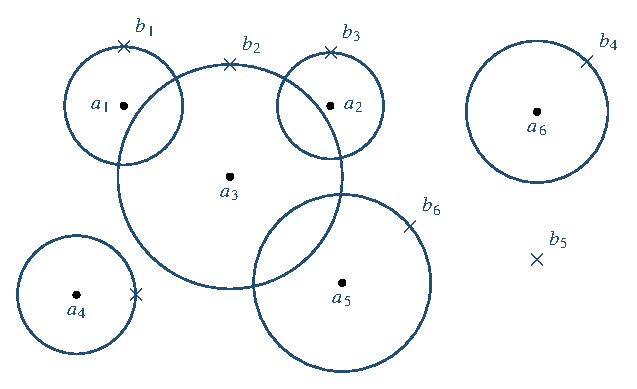
\includegraphics[width=.70\textwidth]{cd1-fig-01.pdf}
\FigureTag{CD1.1}{fig:cd1-01}
\end{figure}
Let dots denote zeros and crosses denote poles. Then $f$ has a power-series expansion in a disc with radius as large as the distance to the pole nearest the centre. But if one wants to study iterates of $f$, one must look at properties preserved by a change of coordinates:
\[
\varphi\circ f\circ\varphi^{-1}\sim f\quad\text{(dynamically)},\qquad
\varphi\circ f^{\circ n}\circ\varphi^{-1}
=(\varphi\circ f\circ\varphi^{-1})^{\circ n}\sim f^{\circ n}.
\]
Zeros and poles are, after all, two points on $\widehat{\mathbb C}$: change coordinates via a M\"obius transformation, and $0,\infty$ go to other points.
% Source page 2
Thus one must look for an invariant of $f$ that is preserved even after a suitable change of coordinates.
\begin{figure}[H]\centering
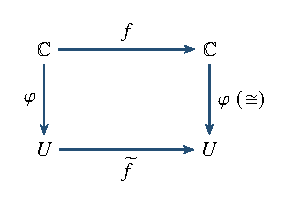
\includegraphics[width=.31\textwidth]{cd1-fig-02.pdf}
\FigureTag{CD1.2}{fig:cd1-02}
\end{figure}
Here $\varphi$ changes coordinates, i.e. it biholomorphically changes the base space. One naturally expects the dynamics to be preserved. Investigation along these lines leads us to two natural invariants: fixed points and critical points.

These invariants organize the study. Dynamics studies the behaviour of the iterates of $f$, especially on sets where small changes in the initial point lead to large changes in its iterated images. More precisely:
\setcounter{definition}{0}\begin{definition}[Fatou set]
Let $f\colon S\to S$ be a holomorphic function on a Riemann surface $S$. A point $z$ belongs to the Fatou set $F$ of $f$ if there is a neighbourhood $U$ of $z$ such that $\{f^{\circ n}|_U\}_n$ is normal.
\end{definition}
\setcounter{definition}{1}\begin{definition}[Julia set]
The set $J=S\setminus F$ is defined to be the Julia set.
\end{definition}
% Source page 3
Motivations aside, when we say that we want to study the dynamics of $f$ on $S$, we essentially want to study the structure of the Fatou and Julia sets of $f$. We do this through fixed points and critical points.
\setcounter{definition}{2}\begin{definition}[Classification of fixed points]
A fixed point $f(\widehat p)=\widehat p$ is
\begin{itemize}
\item attracting if $|f'(\widehat p)|<1$;
\item repelling if $|f'(\widehat p)|>1$;
\item indifferent if $|f'(\widehat p)|=1$.
\end{itemize}
Here $f'(\widehat p)$ means the derivative of the coordinate function of $f$.
\end{definition}
The Fatou and Julia sets are unchanged when $f$ is replaced by an iterate. The next two lemmas make this precise and explain why periodic points may be studied as fixed points of suitable iterates.
\setcounter{theorem}{0}\begin{lemma}[Invariance lemma]\label{cd1:invariance}
For a rational map $f$ of degree at least two, $z\in J(f)$ if and only if $f(z)\in J(f)$.
\end{lemma}
\begin{proof}
It is enough to show $z\in F(f)\Longleftrightarrow f(z)\in F(f)$. If $f(z)\in F(f)$, choose a neighbourhood $V$ of $f(z)$ on which $\{f^{\circ n}\}_n$ is normal, and a neighbourhood $U$ of $z$ with $f(U)\subset V$. Then $\{f^{\circ(n+1)}|_U\}_n$ is normal, and adding the single map $\id|_U$ shows that $z\in F(f)$.

Conversely, suppose $z\in F(f)$. After shrinking a neighbourhood $U$ of $z$, the map $f\colon U\to V=f(U)$ is a proper holomorphic map of finite degree. Normality descends through such a map: if $\{h_n\circ f\}_n$ is normal on $U$, then $\{h_n\}_n$ is normal on $V$. Applying this to $h_n=f^{\circ n}$ shows that $\{f^{\circ n}|_V\}_n$ is normal. Hence $f(z)\in F(f)$.
\end{proof}
The Fatou and Julia sets are invariant under orbits. The next lemma makes this more explicit.
\setcounter{theorem}{1}\begin{lemma}\label{cd1:iterate}
$J(f^{\circ n})=J(f)$.
\end{lemma}
\begin{proof}
By the previous lemma, it suffices to show $F(f^{\circ n})=F(f)$. Certainly $z\in F(f)$ implies $z\in F(f^{\circ n})$. If $z\in F(f^{\circ n})$, there is a neighbourhood $U$ of $z$ such that $\{f^{\circ nm}|_U\}_m\subset K\subseteq\Hol(U,S)$, with $K$ compact. Then
\[
\{f^{\circ m}|_U\}_m\subseteq\bigcup_{i=0}^{n-1}(f^{\circ i}\circ K)
\subseteq\Hol(U,S),
\]
and this finite union is again compact.
\end{proof}
% Source page 5
Passing to an iterate therefore loses no dynamical information. What does it mean to work with fixed points of $f^{\circ m}$?
\setcounter{definition}{3}\begin{definition}[Periodic orbits]
Let $f\colon S\to S$ be holomorphic. An orbit
$f\colon z_0\mapsto z_1\mapsto\cdots\mapsto z_m=z_0$,
with all $z_i$ distinct before returning to $z_0$, is called a periodic orbit of period $m$. Classifying fixed points of $f^{\circ m}$ amounts to dealing with
\[
\lambda=(f^{\circ m})'(z_0)=\prod_{j=0}^{m-1}f'(z_j),
\]
often called the multiplier of the orbit.
\end{definition}
Results stated for fixed points apply to periodic points after passing to the appropriate iterate. We now describe the classification topologically.
% Source page 6
\subsection{Attraction, repulsion, and indifference}
\paragraph{Attraction: multiplier $|\lambda|<1$.}
The following is the topological definition of attraction. Let us first state explicitly the intuitive idea of attraction to a point $\widehat p$. A point $\widehat p\in S$ is said to be attracting if there is a neighbourhood $U$ of $\widehat p$ such that $\{f^{\circ n}|_U\}_n$ converges locally uniformly on $U$ to the constant map $z\mapsto\widehat p$.
\begin{figure}[H]\centering
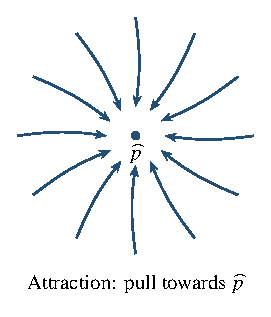
\includegraphics[width=.40\textwidth]{cd1-fig-03.pdf}
\FigureTag{CD1.3}{fig:cd1-03}
\end{figure}
\setcounter{theorem}{2}\begin{lemma}\label{cd1:attraction}
Let $f(\widehat p)=\widehat p$, where $f\in\Hol(S,S)$. Then $|f'(\widehat p)|<1$ if and only if $\widehat p$ is attracting.
\end{lemma}
\begin{proof}
Let $\widehat f$ be the coordinate expression of $f$ locally at $\widehat p$, centred at $\widehat p$. For simplicity assume $\widehat f=f$. If $f(0)=0$ and $|\lambda|=|f'(0)|<1$, analyticity gives $f(z)=\lambda z+O(z^2)$. Thus there is $r_0>0$ such that $|f(z)-\lambda z|=O(|z|^2)$ for $z\in\mathbb D_{r_0}$, and
\[
|f(z)|\le |\lambda z|+C|z|^2\le (|\lambda|+C|z|)|z|.
\]
If $z\in\mathbb D_{r_0}$ is small enough that $|\lambda|+C|z|<1$, then $f$ becomes a contraction mapping, proving that $0$ is attracting.
% Source page 7
One can choose $|\lambda|<c<1$ and $0<r\le r_0$ with $|\lambda|+Cr<c$. In particular, $|\lambda|+C|z|<c<1$ for all $z\in\mathbb D_r$. Hence $|f(z)|<c|z|$, $f(z)\in\mathbb D_r$, and $|f^{\circ n}(z)|<c^n|z|$, so $f^{\circ n}\to(z\mapsto0)$.

Conversely, local uniform convergence to $\widehat p$ implies $(f^{\circ n})'(\widehat p)\to0$. Since $(f^{\circ n})'(\widehat p)=f'(\widehat p)^n$, we obtain $|f'(\widehat p)|<1$.
\end{proof}
Notice that we need holomorphicity of $f$ to conclude that $|\lambda|<1$ is geometrically attracting.

\paragraph{Repulsion: multiplier $|\lambda|>1$.}
This is usually called topological repulsion. Let $f(\widehat p)=\widehat p$. The point $\widehat p$ is repelling if $f$ is locally invertible at $\widehat p$ and $\widehat p$ is attracting for the local inverse fixing $\widehat p$.
\begin{figure}[H]\centering
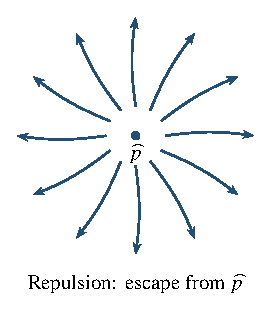
\includegraphics[width=.40\textwidth]{cd1-fig-04.pdf}
\FigureTag{CD1.4}{fig:cd1-04}
\end{figure}
\setcounter{theorem}{3}\begin{lemma}\label{cd1:repulsion}
$|f'(\widehat p)|>1$ if and only if $\widehat p$ is repelling.
\end{lemma}
\begin{proof}
If $|f'(\widehat p)|>1$, then $f$ has a local inverse fixing $\widehat p$ whose multiplier has modulus $|f'(\widehat p)|^{-1}<1$, so the attraction lemma makes $\widehat p$ attracting for that inverse. The converse follows by applying the attraction lemma to the same local inverse.
\end{proof}
% Source page 8
% Source page 9
\paragraph{Indifference: $|\lambda|=1$.}
This does not have an easy-to-visualise topological picture. The indifferent case is treated in \BlogPost{parabolic-fixed-points-and-the-flower-theorem}{\emph{Parabolic Fixed Points and the Flower Theorem}}.

Having seen this, let us collect all points $z\in S$ such that $\{f^{\circ n}(z)\}_n$ converges to an attracting point $\widehat p$. This set is called the \emph{basin of attraction} of $\widehat p$. Such basins belong to the Fatou set; repelling points belong to the Julia set, as do indifferent points of certain kinds. The verification that a basin of attraction lies in the Fatou set is standard.

If $z\in\mathcal A(\widehat p)$, the basin of attraction, then $\{f^{\circ n}(z)\}_n\to z_0$. There is a neighbourhood $U$ of $z_0$ with $U\subset F(f)$, and some $N$ such that $f^{\circ N}(z)\in U$. Hence $f^{\circ N}(z)\in F(f)$, and the invariance lemma gives $z\in F(f)$.

Repelling points lie in the Julia set. Let us introduce a subclass of fixed points, to be taken up in detail later.
\setcounter{definition}{4}\begin{definition}[Parabolic fixed point]
A fixed point $f(\widehat p)=\widehat p$ is parabolic if $f'(\widehat p)$ is a root of unity and $f^{\circ n}\ne\id$ for every $n$.
\end{definition}
% Source page 10
\setcounter{theorem}{4}\begin{lemma}\label{cd1:parabolic}
Parabolic points belong to the Julia set.
\end{lemma}
\begin{proof}
Passing to an iterate, we may assume that the multiplier is $1$.
Locally, $f(w)=w+a_qw^q+a_{q+1}w^{q+1}+\cdots$, so $f^{\circ k}(w)=w+ka_qw^q+\cdots$. Consequently,
\[
\left.\frac{d^q(f^{\circ k})}{dz^q}\right|_0=q!\,ka_q\longrightarrow\infty
\qquad(k\to\infty).
\]
Thus $\{f^{\circ n}\}_n$ cannot converge locally uniformly, for then the sequence of $q$th derivatives at $0$ would also converge.
\end{proof}
Therefore attracting basins lie in the Fatou set, while repelling and parabolic points belong to the Julia set.

Fixed and critical points provide the framework when $f\colon\widehat{\mathbb C}\to\widehat{\mathbb C}$ is rational with $\deg(f)\ge2$.
\subsection{Dynamics of rational maps on the Riemann sphere}
We begin with several general features of Julia sets on the sphere.
% Source page 11
First things first: is $J$ nonempty?
\setcounter{theorem}{5}\begin{proposition}[Nonemptiness]\label{cd1:nonempty}
$J(f)\ne\varnothing$.
\end{proposition}
\begin{proof}
If $J(f)=\varnothing$, there is a sequence $\{n_j\}_j$ such that $\{f^{\circ n_j}\}_j$ converges uniformly on $\widehat{\mathbb C}$ to a rational map $g$, since $\widehat{\mathbb C}$ is compact. For sufficiently large $j$,
\[
\dist(f^{\circ n_j}(z),g(z))<\dist(\text{north pole},\text{south pole})=\pi
\quad(z\in\widehat{\mathbb C}).
\]
Define $H\colon I\times\widehat{\mathbb C}\to\widehat{\mathbb C}$ by
$H(t,z)=\gamma_{g(z)\to f^{\circ n_j}(z)}(t)$, where $\gamma$ is the unique geodesic path between those two points. Since $\gamma_{a\to b}$ is continuous in both $a$ and $b$, $H$ is continuous. Thus $f^{\circ n_j}$ and $g$ are homotopic. Homotopic self-maps of the sphere have the same topological degree, giving $\deg(f^{\circ n_j})=\deg(g)$. But $\deg(f^{\circ n_j})\to\infty$ as $j\to\infty$, a contradiction.
\end{proof}
We next distinguish periodic orbits from eventually periodic orbits.
\setcounter{definition}{5}\begin{definition}[Grand-orbit-finite points]
For $z\in S$, define
\[
\operatorname{GO}(z,f)=\{z'\in S:\operatorname{orbit}(z)\cap\operatorname{orbit}(z')\ne\varnothing\}.
\]
A point whose grand orbit is finite is called \emph{exceptional}.
% Source page 12
The set of all such points is denoted by $\mathcal E(f)$ and called the grand-orbit-finite set. The set $\operatorname{GO}(z,f)$ is the grand orbit of $z$.
\end{definition}
Exceptional points are severely constrained:
\setcounter{theorem}{6}\begin{lemma}\label{cd1:exceptional}
$|\mathcal E(f)|\le2$. All exceptional points are superattracting.
\end{lemma}

\begin{proof}
For $z\in\mathcal E(f)$, $\operatorname{GO}(z,f)$ is a single periodic orbit; otherwise one can keep tracing back. For any $\widehat z\in\widehat{\mathbb C}$, $f^{-1}(\widehat z)$ has $d$ preimages counted with multiplicity, since
\[
f(z)=\frac{P(z)}{Q(z)}=\widehat z
\quad\Longleftrightarrow\quad P(z)-\widehat zQ(z)=0
\]
has $d$ zeros counted with multiplicity. If the multiplicity of $z_j\in f^{-1}(\widehat z)$ is greater than one, then $z_j$ is critical: the order of the zero of $f(z_j)-\widehat z$ is greater than one, so $f'(z_j)=0=(f(z_j)-\widehat z)'$.

Write $\operatorname{GO}(z,f)=\{a_0\mapsto a_1\mapsto\cdots\mapsto a_m=a_0\}$. Clearly all $a_i$ are superattracting, so $a_i\in F(f)$ and $\mathcal E(f)\subset F(f)$. If $|\mathcal E(f)|\ge3$, let $U=\widehat{\mathbb C}\setminus\mathcal E(f)$. Then $U$ is hyperbolic and $f(U)=U$, so $\{f^{\circ n}|_U\}_n$ is normal. This gives $U\subset F(f)$ and $J(f)=\varnothing$, a contradiction.
\end{proof}
% Source page 13
\setcounter{theorem}{7}\begin{proposition}[Expansion]\label{cd1:expansion}
Let $z\in J$. If $N$ is a neighbourhood of $z$, then
\[
\bigcup_{n\ge0}f^{\circ n}(N)\supseteq\widehat{\mathbb C}\setminus\mathcal E(f).
\]
Equality holds for sufficiently small $N$.
\end{proposition}
\begin{proof}
If $U=\bigcup_{n\ge0}f^{\circ n}(N)$ omits three points, note that $f(U)\subseteq U$. Since $U$ is hyperbolic, $\{f^{\circ n}|_U\}_n$ is normal, so $z\in F(f)$, a contradiction. Thus $|\widehat{\mathbb C}\setminus U|\le2$. As $f(U)\subseteq U$, the points in $\widehat{\mathbb C}\setminus U$ must belong to the grand-orbit-finite set. Finally, equality holds if $N\subset\widehat{\mathbb C}\setminus\mathcal E(f)$.
\end{proof}
\setcounter{theorem}{8}\begin{proposition}[Empty interior]\label{cd1:interior}
If $\operatorname{Int}(J)\ne\varnothing$, then $J=\widehat{\mathbb C}$.
\end{proposition}
\begin{proof}
If $\operatorname{Int}(J)\ne\varnothing$, there is a point $z$ with a neighbourhood $N\subseteq J$. By the invariance lemma, $\bigcup_n f^{\circ n}(N)\subseteq J$. Since $J$ is closed,
$J\supseteq\overline{\widehat{\mathbb C}\setminus\mathcal E(f)}=\widehat{\mathbb C}$, giving the assertion.
\end{proof}
% Source page 14
Within attracting basins, open sets shrink under iteration, whereas near the Julia set they expand to cover almost all of $\widehat{\mathbb C}$. Let us put these two concepts together.
\setcounter{theorem}{9}\begin{proposition}[Basin boundary equals Julia set]\label{cd1:boundary}
If $\mathcal A$ is an attracting basin, then $\partial\mathcal A=J$.
\end{proposition}
\begin{proof}
The Julia set expands open sets around it. If $z\in J(f)$ and $N$ is a neighbourhood of $z$, some iterate $f^{\circ k}(N)$ meets $\mathcal A$. By complete invariance, $N$ itself meets $\mathcal A$. Since $J(f)\cap\mathcal A=\varnothing$, this gives $J(f)\subseteq\partial\mathcal A$.

On the other hand, $\mathcal A$ is a union of Fatou components. Indeed, if one point of a Fatou component belongs to $\mathcal A$, normality and the identity theorem show that every point of that component converges to the same attracting cycle. No point of the open set $F(f)$ can therefore lie on $\partial\mathcal A$. Hence $\partial\mathcal A\subseteq J(f)$, and $\partial\mathcal A=J(f)$.
\end{proof}
\begin{remark}
This property essentially spells out the nature of the dynamics of $f$. An attracting basin has connected components, or islands, separated by a thin set $J$ (it has no interior). The connected components of the Fatou set are called the Fatou components of $f$.
\end{remark}
% BLOG-CONTENT-END
\bibliographystyle{amsalpha}
\bibliography{tools/profiles/complex-dynamics-notes/references}
\end{document}
